\section{Literature review}\label{sec:review}

This section comprises what could be considered a classical literature review:
an analysis of selected articles and publications that constitute the state and
progress of each research topic.

% TODO Would a diagram of some sort be nice here?

\subsection{Clustering}\label{subsec:clustering}
\graphicspath{{img/clusters/}}

Clustering, or \emph{cluster analysis}, is a generic term used to describe a
number of techniques whose objective is to partition some dataset into parts
(clusters) according to some distance (similarity) measure. The generated
partition should be such that the members of one cluster are more similar to one
another than the rest of the data~\cite{Everitt2011}. This form of analysis has
found applications in a multitude of fields, including recently the optimisation
of energy systems~\cite{Jing2019,Teichgraeber2019}, wireless sensor
networking~\cite{Goswami2019}, and the biological
sciences~\cite{Bulut2020,Kiselev2019}.

Clustering originated in the social sciences around the turn of the
20\textsuperscript{th} century in a similar manner to several other (now
ubiquitous) statistical tools, including hypothesis testing and \(p\)-values,
correlation, and factor analysis. Early work on cluster analysis, such
as~\cite{Cattell1943,Driver1932}, focused on its applications in attempting to
identify traits which led to cultural and psychological differences between
groups of people, as opposed to studying the methods used to identify any
partitions.

The focus of clustering research shifted to the statistical nature of the
methods following work on clustering under the name \emph{numerical
taxonomy}~\cite{Sneath1973,Sokal1966}. These works were highly influential and
led to an abundance of research into clustering methods,
including~\cite{Diday1976} and~\cite{Hartigan1975} which each formalised the
principles of clustering as a part of statistics. Furthermore, this period
witnessed the advent of seminal work on clustering algorithms such as
\(k\)-means~\cite{Hartigan1979} and hierarchical
clustering~\cite{Defays1977,Sibson1973} that are still considered fundamental
methods.
% TODO Can we have a reference or 2 here to backup claim that they're
% still fundamental? (Perhaps even the initialisation paper of yours.
Since then, with an increase in the data under study, clustering has fallen more
squarely into the category of machine learning techniques that perform
\emph{unsupervised learning} --- this is because clustering relies solely on the
entirety of the observed data and some a priori knowledge such as a set of
parameters~\cite{Dayan1999}.

The remainder of this section offers a summary of the three principle types of
clustering algorithms: those belonging to the \(k\)-means (centroid-based)
paradigm, hierarchical models, and, finally, density-based algorithms. In
addition to these, fuzzy clustering and model-based clustering are popular. For
overviews and reviews of the methods belonging to the former,
consider~\cite{Ferraro2019,Gosain2016,Li2016},
and~\cite{Bouveyron2019,Fruhwirth2019,McNicholas2016} for the latter.

\subsubsection{Centroid-based clustering}\label{subsubsec:kmeans}

The concept of \(k\)-means clustering is to partition a
real-valued dataset into \(k \in \mathbb N\) homogeneous parts (clusters), where
each data point is assigned to the cluster to which the point is closest. The
sum of these within-cluster distances is often referred to as the \emph{inertia}
of the clustering. The distance from a point to a cluster is defined as the
distance from the point to the mean of the elements in that cluster, also
referred to as the cluster centre or centroid; this alternative name gives
another name to the paradigm, \emph{centroid-based clustering}. Typically, the
distance measure used is the Euclidean distance, with the assumption that
several preprocessing techniques are used to mitigate any scaling discrepancies
in the attributes of the data.

Although \(k\)-means clustering has independently been discovered a number of
times since as early as the 1950s (comprehensive histories on the subject can be
found in~\cite{Bock2007,Jain2010}), its formulation is commonly attributed
to~\cite{Hartigan1979}. Given its lengthy standing, there are a multitude of
algorithms that perform \(k\)-means clustering. However, the most commonly used
is Lloyd's algorithm~\cite{Lloyd1982}. This procedure is remarkably
uncomplicated in its statement, and has now become so synonymous with
\(k\)-means clustering that it is referred to as `the \(k\)-means algorithm'. To
summarise it in a sentence, the algorithm iteratively partitions the numerical
data into \(k\) parts, reassigning data points and adjusting cluster means until
no point moves cluster on a full cycle of the dataset. The algorithm has proven
popular due to this simplicity. Furthermore, it is scalable and can be
parallelised~\cite{Bahmani2012}, and its implementations are
concise~\cite{Olafsson2008,Wu2009}.

However, centroid-based clustering is not without its drawbacks. The most
notable of these is its dependency on being presented with data that can be
naturally partitioned into \(k\) clusters of a particular
type~\cite{Ostrovsky2013}. Namely, the true clusters should be isotropic, convex
and linearly separable. The reason these conditions exist, particularly for
\(k\)-means, is because the \(k\)-means (Lloyd's) algorithm is a heuristic for
identifying the centroidal Voronoi tessellation of a dataset~\cite{Du2006}.
Hence, the true objective of the algorithm is to divide the attribute space into
\(k\) equally weighted parts using the dataset as a sample, rather than focusing
on dividing the dataset itself.

Regardless of the true nature of a centroid-based clustering algorithm, there is
the issue of choosing a suitable value of \(k\) prior to clustering. A common
approach to this problem is the so-called `elbow' method where a clustering
algorithm is run using a range of values for \(k\)~\cite{Aggarwal2013}. This
range is typically informed by what is considered reasonable in the problem
domain. From these runs, the value of \(k\) is plotted against some objective
and the plot is inspected for a kink or `elbow'. Typically, inertia is used, but
another popular metric is the silhouette coefficient: a measure for both the
intra-cluster tightness and inter-cluster separation of a
clustering~\cite{Rousseeuw1987}.

Irrespective of the objective used, the definition of what constitutes an elbow
is not necessarily well-defined. The works \cite{Sujatha2013,Syakur2018} each
employ the elbow method with final inertia as the objective. In each case, the
authors offer little explanation of their methodologies other than choosing
\(k\) where `drastic' changes occur in the objective. Attempts to formalise this
method have been made, however. For instance, the authors of \cite{Satopaa2011}
provide a `knee-point' detection algorithm that finds the point of maximal
curvature in the domain of a function when provided with some basic properties
of that function (whether it is convex, monotonic, etc.). This algorithm has
been adapted to cleanly carry out the elbow method in software packages, such as
Yellowbrick~\cite{Bengfort2019}, by interpolating the objective values.

Further to this formalisation of the elbow method, other extensions to
\(k\)-means itself have been presented to alleviate all dependency on making a
choice for \(k\). For example, in~\cite{Olukanmi2019}, the authors propose an
automatic decision scheme for \(k\)-means based on a vector comprised of the
values that constitute the inertia of a clustering. The process determines that
if this vector meets some criterion attached to its standard deviation, then
each cluster is sufficiently unimodal and Gaussian, fulfilling the condition
that clusters be roughly spherical.

Another limitation of \(k\)-means is that it is dependent on its initial
solution. The standard initialisation process is to select \(k\) points in the
dataset at random, introducing a stochastic element to the algorithm. Studying
methods to find sensible (ideally, deterministic) initial solutions has formed a
substantial part of centroid-based clustering research. For instance, the
authors of~\cite{Manoharan2016} provide a novel initialisation that pursues the
Voronoi tessellation by use of a `divide-and-conquer' approach. Under the
presented scheme, the initial centroids are selected based on a rough partition
of the attribute space according to their extreme values.  Likewise, the
initialisation presented in \cite{Singh2013} assigns each centroid using the
arithmetic mean and dividing the remaining attribute space in two.  Meanwhile,
the method introduced in~\cite{Katara2015} initialises \(k\)-means by sorting
the instances in the dataset according to their distance from the origin. Once
sorted, the instances are split into \(k\) disjoint sets and the mean of each
set is assigned as a centroid. A likely issue with this approach is that there
are new assumptions about the data, i.e. that it is centred about the origin in
all dimensions (rectifiable through feature scaling), and that all points
equidistant from the origin are similar to one another.

A crucial part of centroid-based clustering research is dedicated to alternative
measurements for the centre of a cluster. A cluster centroid is broadly regarded
as a purely geometric object, and is measured using a distance metric and a
measure of central tendency. Using the Euclidean mean as the centre of a cluster
is a sensible choice when clustering continuous, normalised data. However, if
the data is not scalable (if it is categorical, for instance) then this approach
is not suitable. Further, the Euclidean distance is linear, leading \(k\)-means
to be prone to the effects of outliers in the data. As such, numerous
extensions to Lloyd's algorithm exist in the literature that are designed to be
more robust to these limitations. For continuous (or at least ordered) data,
\(k\)-medians and \(k\)-medoids exist. The former uses the median value of each
attribute in a cluster to form the centre~\cite{Arya2001,Bradley1997},
mitigating the effect of outliers.

In \(k\)-medoids, the centre of a cluster is taken to be the data point
which is closest to all other points in the cluster~\cite{Kaufman1987}.
Typically, \(k\)-medoids makes use of the Manhattan distance, but is generic in
its schema. If Euclidean distance is used, then \(k\)-medoids is identical to
\(k\)-means, with the restriction that the centre of the cluster is an actual
point in that cluster. Specifying that the centre be a real point is seen as the
primary benefit of \(k\)-medoids, and continues to be actively
studied~\cite{Schubert2019,Ushakov2021}. There are cases where a virtual cluster
centre is not sufficient, such as facility allocation~\cite{Chen2016,Wang2020}
and the clustering of gene sequences~\cite{Johnson2018}.

When considering a categorical or mixed-type dataset, none of the aforementioned
clustering techniques will work as they were intended because the sense of order
does not exist across the entire attribute space. While it is possible to use
\(k\)-means in these situations, by converting any categorical attributes into
pseudo-numerical (binary) attributes by use of dummy coding, this is not
recommended. One potential failing is the inflated effect of categorical
variables with many distinct values in any distance calculation, as these will
produce more binary variables. Another is that by introducing potentially many
binary variables, the dimensionality of the dataset increases substantially, and
so the points in the higher-dimension form of the data become intrinsically
further from one another, thus loosening any sense of cluster homogeneity.

Therefore, another approach should be taken that handles the data directly. The
\(k\)-modes and \(k\)-prototypes algorithms (introduced in~\cite{Huang1998}) are
capable of handling categorical and mixed-type data, respectively. The
\(k\)-modes algorithm is an extension to Lloyd's algorithm, like \(k\)-medians
and \(k\)-medoids, where the cluster centre is defined as a point whose
attribute values are most frequent among those of the points in a
cluster.~\cite{Huang1998} provides a so-called `matching dissimilarity' measure
to expedite the centre calculations, making \(k\)-modes scalable and
computationally efficient~\cite{Madhuri2014}. The \(k\)-prototypes algorithm is
essentially a blended form of \(k\)-modes and \(k\)-means where each method is
applied to the categorical and numeric attributes at each iteration, before
their respective costs are combined linearly according to some parameter,
\(\gamma\). Work into \(k\)-modes clustering is largely focused on the initial
choice of centroids, as
in~\cite{Cao2009,Jiang2016,Khan2013,Khan2007,Taoying2013,Wilde2020}, and
improving on the original distance measure. Two popular dissimilarity measures
for \(k\)-modes clustering were presented in~\cite{Cao2012} and~\cite{Ng2007}.
Each of these novel measures improve on the basic metric by taking into account
the relative frequency of the values of each attribute. The latter
measure~\cite{Ng2007} focuses locally to the cluster at hand, while the
former~\cite{Cao2012} considers their frequencies from a universal perspective.

While centroid-based clustering is dominated by Lloyd-like algorithms, recent
work has sought out alternative approached. For instance, the authors
of~\cite{Chen2019} revise centroid clustering from an expectation-maximisation
process to one that considers its data points as agents that act with
preferences based on their locale. The overall aim of this approach is to
incorporate a sense of mathematical fairness by identifying a solution that can
not be justifiably rejected by any subset of its agents. Such a solution is
found through a proportional (i.e. Pareto-optimal) distribution of the cluster
centres according to some distance metric.

At this point, the survey returns to the effect of outliers on Lloyd-like
algorithms, especially \(k\)-means, and the literature around reducing that
effect. The \(k\)-means-sharp algorithm was presented in~\cite{Olukanmi2017};
this revision to \(k\)-means embeds an outlier detection feature which relies
solely on the underlying structures from the original \(k\)-means algorithm. The
benefit of handling adverse noise in this way is twofold: first, it preserves
the computational efficiencies that come with using the mean (as opposed to
sorting the attributes of each cluster to find a median in \(k\)-medians, say);
and, second, there are no additional parameters to determine.
In~\cite{Gupta2017}, the authors provide another integration with \(k\)-means
for detecting outliers by way of a local search, but in order to do so, they
introduce another parameter determining the cardinality of the neighbourhood of
a point. In contract to these extensions, are examples of works that exploit
this weakness of \(k\)-means clustering~\cite{Lei2012,Wei2019}. In each case,
the \(k\)-means algorithm partitions a dataset, and outliers are identified
according to some neighbourhood threshold associated with the elements of a
cluster.

The final remark in this section of the survey is concerned with the relaxation
of the constraints on cluster geometry by centroid-based clustering algorithms.
This particularity is fundamental to how these algorithms operate and are
designed, and so little research has been done on the subject. Having said that,
the work in~\cite{Sung1998} demonstrates how the Mahalanobis distance can be
used in place of the Euclidean distance to circumvent the dependency on
spherical (i.e.  isotropic) clusters by \(k\)-means. However, the resultant
clusters must still be convex and linearly separable. The Mahalanobis distance
is commonly used to detect outliers in other settings, and is dependent on the
eigenvalues of the covariance matrix derived from a
dataset~\cite{Mahalanobis1936}. A potential downside to this measure is the
singularity of that matrix, which is particularly likely in high-dimensional
data. Another exemplar work is~\cite{Statman2020}, where a variant of
\(k\)-means is presented as being agnostic to its distance measure, and removes
the requirement for the attribute space to be a metric space at all.

\begin{table}
    \begin{tabular}{llrccc}
\toprule
{} &                      Summary &  No. clusters &  Convex & Separable & Isotropic \\
\textbf{Name    } &                              &               &         &           &           \\
\midrule
\textbf{Moons   } &  Interlocking crescent moons &             2 &  \xmark &    \xmark &    \xmark \\
\textbf{Ellipses} &           Elongated globules &             3 &  \cmark &    \cmark &    \xmark \\
\textbf{Spheres } &            Rough-edged balls &             4 &  \cmark &    \cmark &    \cmark \\
\bottomrule
\end{tabular}

    \caption{A summary of the synthetic datasets}\label{tab:datasets}
\end{table}

Figure~\ref{fig:kmeans_examples} demonstrates the nuances of centroid-based
clustering discussed in this section, and shows how the \(k\)-means algorithm
performs on three synthetic datasets. A brief summary of these datasets is
provided in Table~\ref{tab:datasets}. The datasets were created using the Python
library Scikit-learn~\cite{scikit-learn}, and the source code to generate them
(and the plots included in this survey) is available at the GitHub repository
for this manuscript (\url{github.com/daffidwilde/literature-review}), and has
also been archived online under~\doi{10.5281/zenodo.4320050}.

\begin{figure}
    \centering
    \begin{subfigure}{.333\textwidth}
        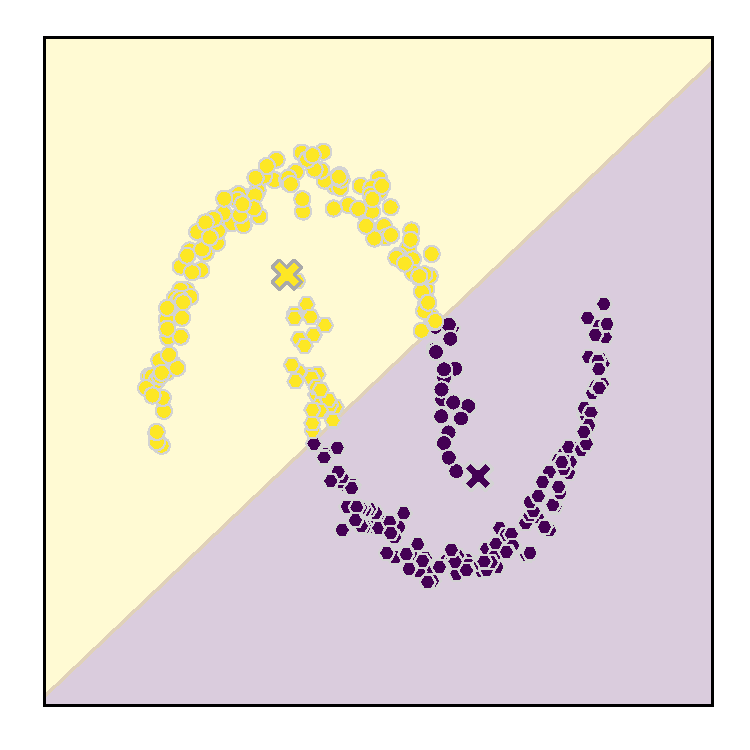
\includegraphics[width=\linewidth]{kmeans/moons}
        \caption{}\label{fig:kmeans_moons}
    \end{subfigure}%
    \hfill%
    \begin{subfigure}{.333\textwidth}
        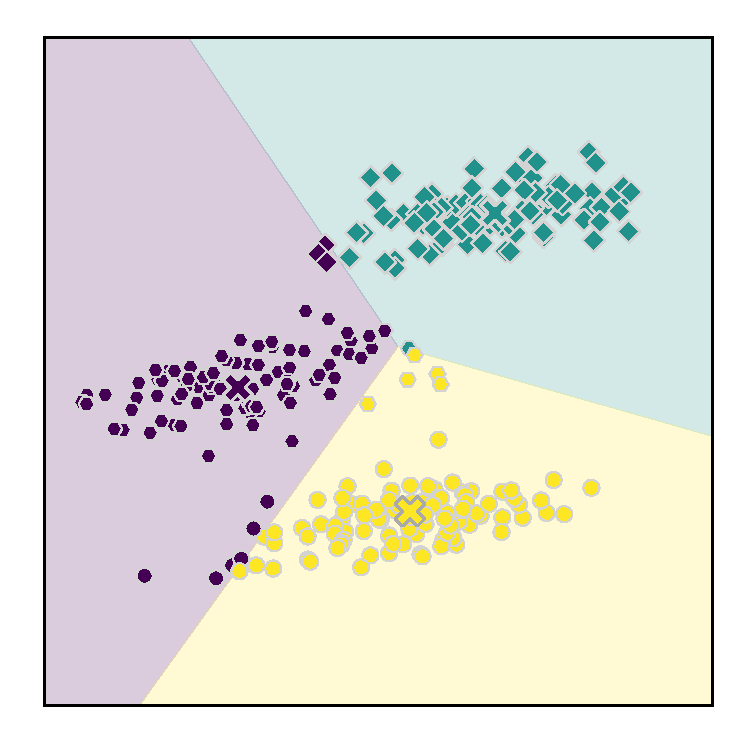
\includegraphics[width=\linewidth]{kmeans/ellipses}
        \caption{}\label{fig:kmeans_ellipses}
    \end{subfigure}%
    \hfill%
    \begin{subfigure}{.333\textwidth}
        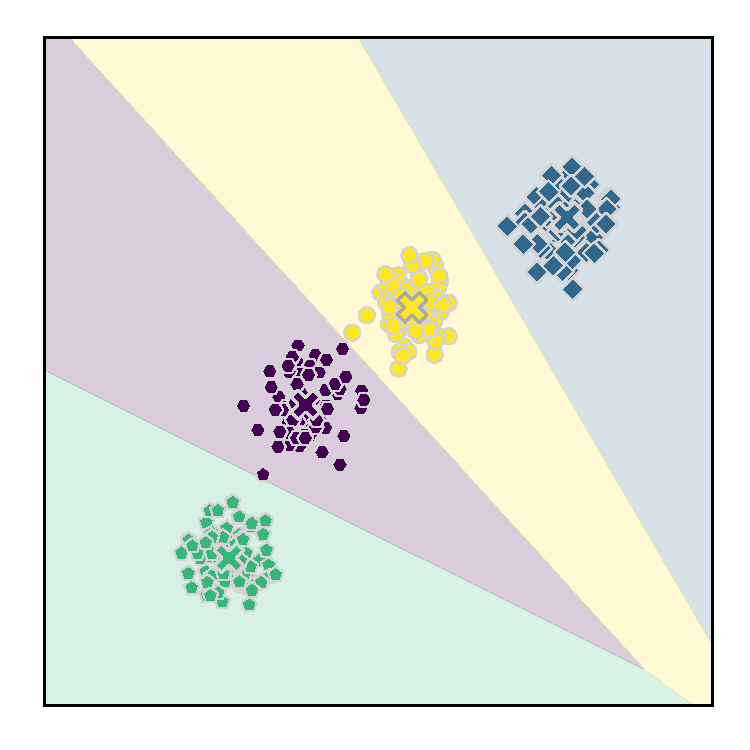
\includegraphics[width=\linewidth]{kmeans/spheres}
        \caption{}\label{fig:kmeans_spheres}
    \end{subfigure}
    \caption{%
        Clusters identified by \(k\)-means on the (\subref{fig:kmeans_moons})
        moons, (\subref{fig:kmeans_ellipses}) ellipses, and
        (\subref{fig:kmeans_spheres}) spheres datasets.%
    }\label{fig:kmeans_examples}
\end{figure}

Each plot in the figure shows a grouped scatter plot of the identified clusters,
with the true clusters indicated by the marker shape. In addition to this
scatter, the cluster centres are shown (as crosses), as well as the Voronoi
cells defined by those centres (as shaded regions). Note that the axes are
presented without labels. The name and scale of each attribute detracts from the
purpose of this figure, which is to demonstrate the clustering. As such, all
unnecessary information has been removed.

Figure~\ref{fig:kmeans_moons} shows a stark example of where centroid-based
clustering fails; despite the clusters in the dataset being distinct,
\(k\)-means is unable to identify them. Instead, the attribute space is divided
to create two equally weighted regions. Likewise, in
Figure~\ref{fig:kmeans_ellipses}, the placement of the cell boundaries has been
determined by weighting, rather than the cluster locations. Finally, with
Figure~\ref{fig:kmeans_spheres}, \(k\)-means performs well, correctly
partitioning the dataset into its four clusters.

\subsubsection{Hierarchical clustering}

Hierarchical clustering seeks to identify a hierarchy of the relationships
between subsets of points in a dataset. A hierarchical clustering algorithm
depends on a distance metric for measuring inter-point similarity, and a
\emph{linkage criterion} to determine the distance between two sets of points.
For the most part, algorithms for hierarchical clustering are one of two types:
agglomerative or divisive~\cite{Kaufman1990}. Agglomerative algorithms,
originating with~\cite{Johnson1967,Ward1963}, begin with each point in its own
cluster and work to merge clusters together, constructing the hierarchy from the
bottom up. Meanwhile, divisive algorithms, with~\cite{Edwards1965} being an
early example, take a top-down approach and seek to split the dataset into
reasonably homogeneous clusters.

Since its origins, hierarchical clustering research has been dominated by
agglomerative methods; this is due, largely, to the computational issues
associated with how to best split a heterogeneous dataset into parts
recursively. For a dataset of \(n\) points, a complete search of the possible
splits takes \(2^n\) calculations, and so divisive methods require efficient
heuristics to be even remotely plausible on real-world data. A common choice is
the \(k\)-means algorithm~\cite{Moseley2017,Peterson2018} which was discussed in
Section~\ref{subsubsec:kmeans}.

In addition, hierarchical clustering has been successfully reframed as a
combinatorial optimisation problem, as is done with divisive clustering
in~\cite{Dasgupta2016}, which allows for the application of optimisation
heuristics such as linear programming~\cite{Roy2017}, local
search~\cite{Aljarah2019} and probabilistic estimation~\cite{Fan2015} to
identify a clustering in reasonable time. Furthermore, related works exist which
concern themselves with determining the quality of a hierarchical structure with
respect to some cost function, like~\cite{Bilu2012,Lyzinski2017}.
In~\cite{CohenAddad2018}, the authors combine these methodologies to produce a
divisive clustering algorithm that achieves logarithmic complexity.

While heuristic methods exist for agglomerative
clustering~\cite{Aljarah2019,Fan2015}, its methods do not bear the same burdens
as divisive methods; the grouping together of parts can be achieved with more
straightforward tools. Generally, the definition of an agglomerative
algorithm is reliant on their linkage criterion. Meanwhile, the
distance metric used is largely dependent on the type of data
presented~\cite{Nielsen2016}. Two of the fundamental criteria for hierarchical
clustering are complete linkage, which defines the CLINK
algorithm~\cite{Defays1977}, and single linkage, providing the SLINK
algorithm~\cite{Sibson1973}. For two clusters, \(X\) and \(Y\), and a point-wise
distance metric, \(d\), each criterion, \(D\), is evaluated as follows:

\begin{itemize}
    \item Complete linkage: \(D(X, Y) = \max_{x \in X, y \in Y} d(x, y)\)
    \item Single linkage: \(D(X, Y) = \min_{x \in X, y \in Y} d(x, y)\)
\end{itemize}

These definitions give each approach the colloquial names \emph{farthest
neighbour} and \emph{nearest neighbour} clustering, respectively. Another
popular linkage criterion is average-linkage, which defines the distance between
two clusters as the mean distance between any point in one cluster and any point
in the other. Defining linkage criteria with point-wise distances allows a
hierarchical (agglomerative or divisive) algorithm to be run using only a
point-wise distance matrix, as opposed to a dataset directly, allowing for
increases in computational efficiency by use of caching~\cite{Nielsen2016}.
However, hierarchical methods continue to be prone to outliers and are biased
towards globular clusters because of definitions such as these. Ongoing reviews
on the subject of hierarchical (although predominantly agglomerative) clustering
methods are available~\cite{Murtagh1983,Murtagh2012,Murtagh2017}.

Like centroid-based clustering, a principle issue with hierarchical clustering
is knowing how many clusters is the most appropriate number. Hierarchical
algorithms terminate when all points exist in a single cluster (for
agglomerative methods) or are all separate (for divisive). A key advantage of
clustering in this way is the retention of a complete history of how the points
relate to one another. These histories are used to visualise the clustering
process via a dendogram. A dendogram is an acyclic graph (tree) arranged into
levels corresponding to the stages at which two clusters are merged (or split).

With such a visualisation, and the underlying tree itself, an appropriate number
of clusters can be identified after running the algorithm once, as opposed to
the ranges of runs required for the elbow method in centroid-based clustering.
The authors of~\cite{Tellaroli2016} present a hierarchical clustering schema
that incorporates complete-linkage clustering with the minimum variance
criterion presented in~\cite{Ward1963}. In doing so, the method automates the
process of choosing an appropriate number of clusters; a decision that is
usually made post hoc according to another metric, such as the silhouette
coefficient, evaluated at each level of the tree.

Figure~\ref{fig:hierarchical_examples} shows the output of agglomerative
clustering with average linkage on the three synthetic datasets described in
Table~\ref{tab:datasets}. For each example, both the grouped scatter plot (left)
and a dendogram (right) are shown. To obtain the scatter plot, the clustering
was stopped when the required number of clusters had been identified. The same
clustering can be identified by drawing a horizontal line on the dendogram at
the level where the number of vertical links equals the number of clusters. The
subtrees below that line form the clusters in the scatter plot. In the figure,
this level has been indicated by colouring the requisite links with the
corresponding cluster colour. Note again, that the figures are deliberately bear
to focus on the outcome of the clustering, rather than the artificial attribute
values.

\begin{figure}
    \centering
    \begin{subfigure}{\textwidth}
        \centering
        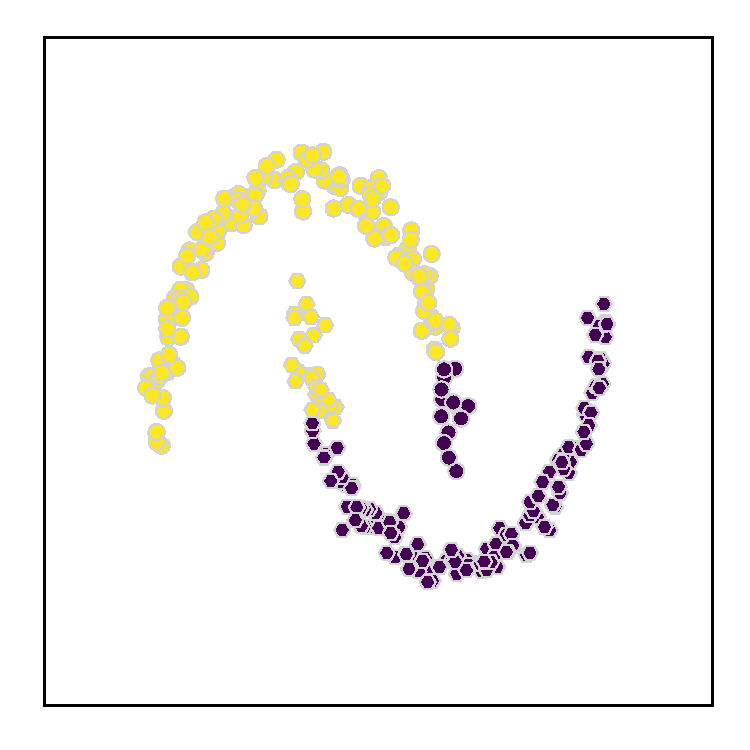
\includegraphics[height=\hierheight]{hierarchical/moons}
        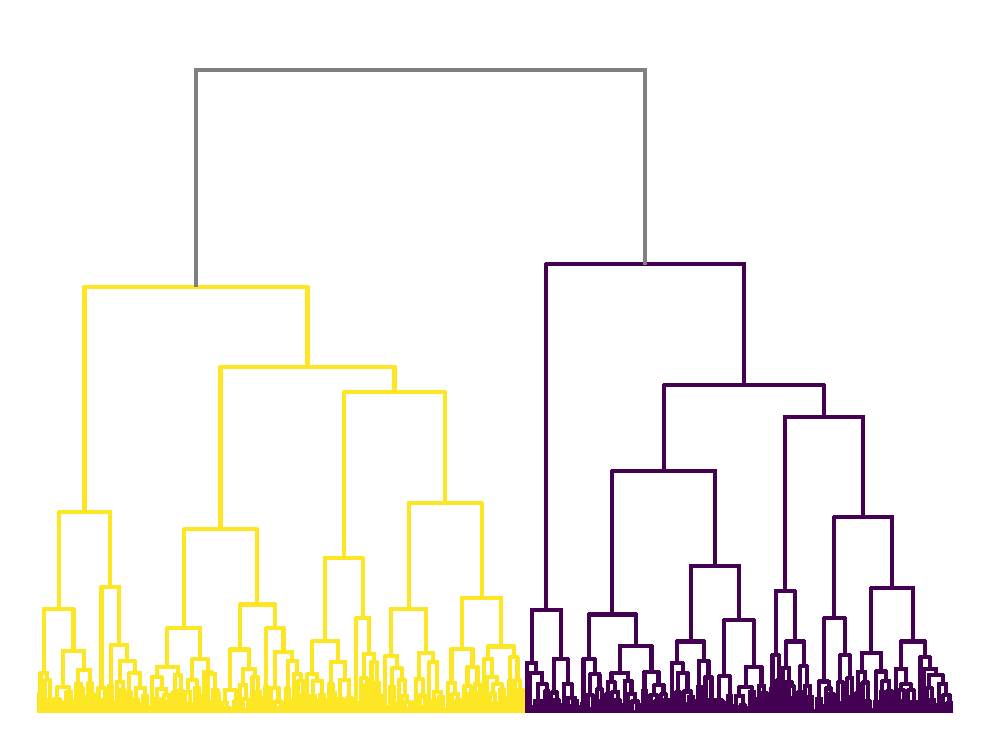
\includegraphics[height=\hierheight]{dendogram/moons}
        \caption{The moons dataset}\label{fig:hierarchical_moons}
    \end{subfigure}

    \begin{subfigure}{\textwidth}
        \centering
        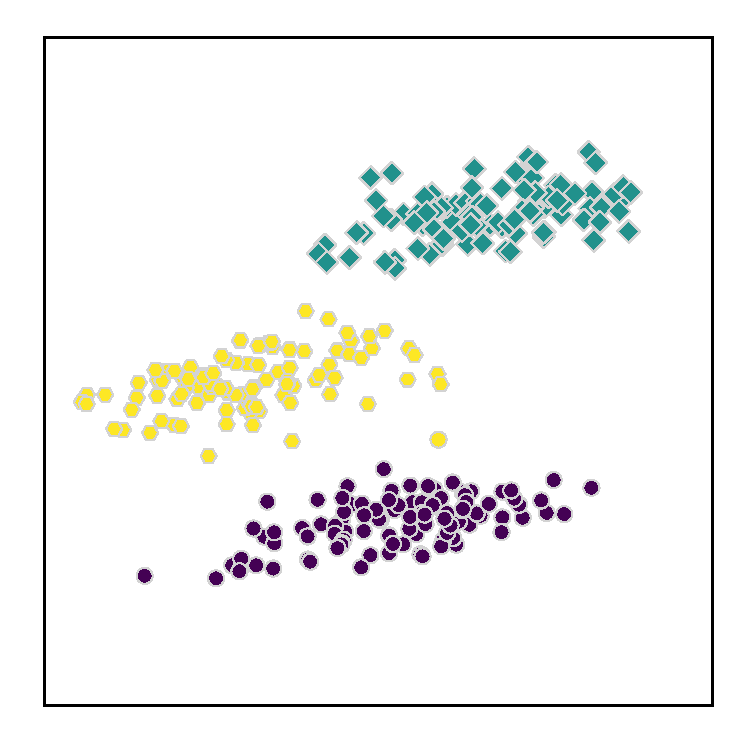
\includegraphics[height=\hierheight]{hierarchical/ellipses}
        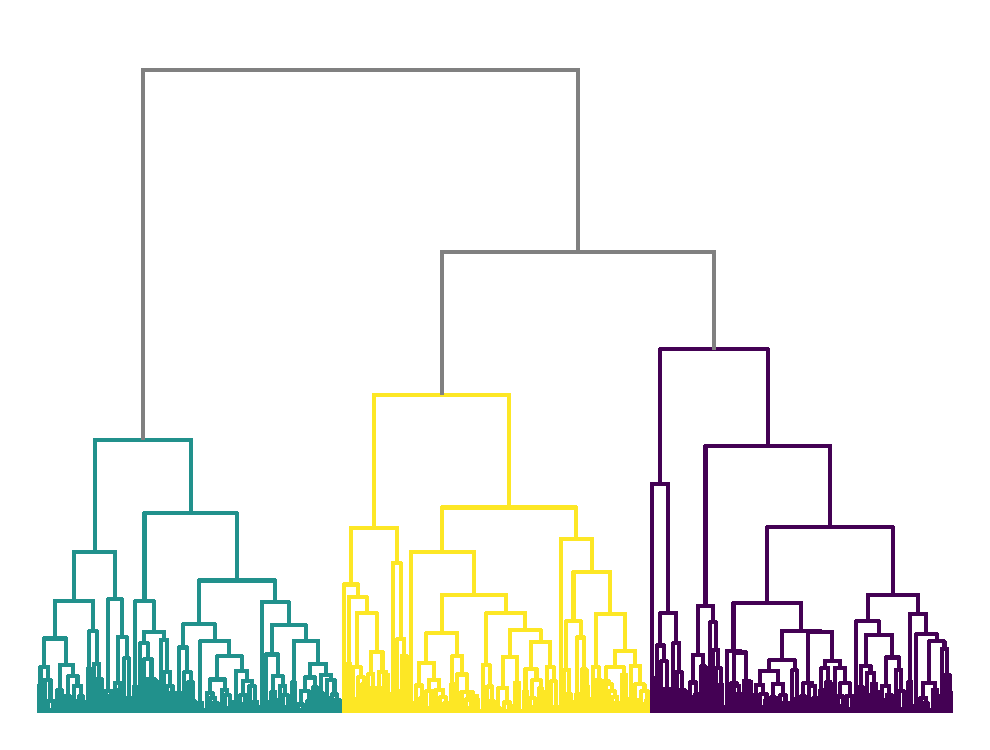
\includegraphics[height=\hierheight]{dendogram/ellipses}
        \caption{The ellipses dataset}\label{fig:hierarchical_ellipses}
    \end{subfigure}%

    \begin{subfigure}{\textwidth}
        \centering
        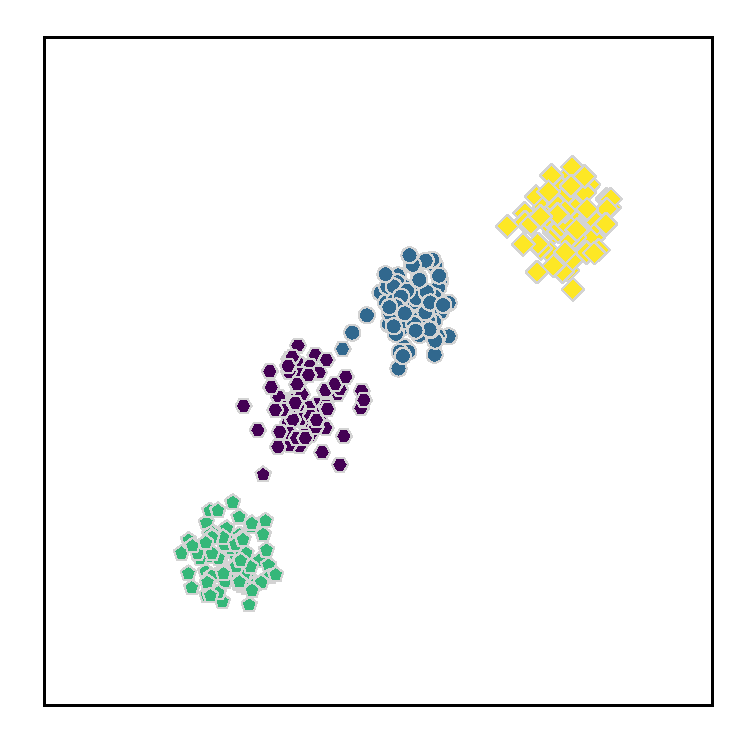
\includegraphics[height=\hierheight]{hierarchical/spheres}
        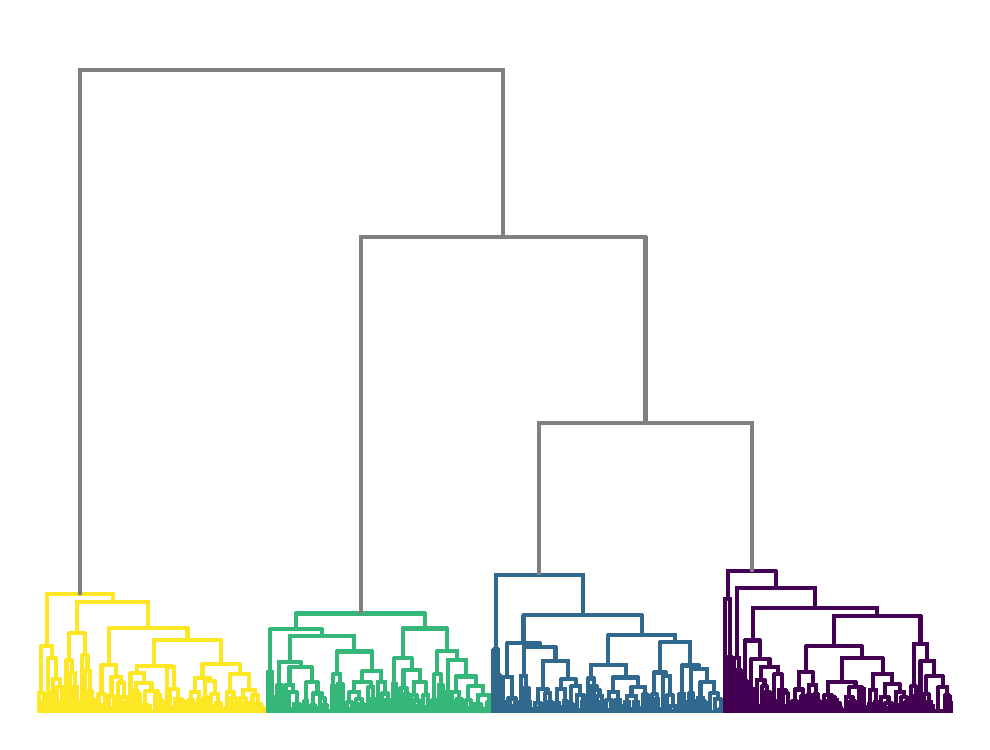
\includegraphics[height=\hierheight]{dendogram/spheres}
        \caption{The spheres dataset}\label{fig:hierarchical_spheres}
    \end{subfigure}
    \caption{%
        Clusters and dendograms identified by average-linkage clustering on the
        synthetic datasets.%
    }\label{fig:hierarchical_examples}
\end{figure}

Like \(k\)-means, average-linkage clustering struggled to identify the moons in
Figure~\ref{fig:hierarchical_moons}, but other linkage criteria may be robust to
shapes such as these. For the remaining examples, hierarchical clustering
appears to perform well at identifying convex, linearly separable regions in the
datasets. However, there are a handful of incorrectly clustered points along the
borders of some regions.

\subsubsection{Density-based clustering}

Density-based clustering differs from centroid-based methods in that
it actively seeks more of the underlying structure of a dataset. In
centroid-based clustering, decisions are made using the distance between two
points, which provides a \emph{flat} clustering without an underlying structure.
Meanwhile, hierarchical methods make use of identification and aggregation
devices, which are derived from point-wise distances, to measure and organise
the connectivity of subsets in a dataset, providing insight into the structure
of the data. Arguably, density-based clustering takes this structural approach a
step further and considers the attribute space of a dataset as a density
surface. Then, a cluster is defined as a high-density region of that surface.

By considering a dataset in this way, the clusters can be of arbitrary shape,
overcoming the major shortfall of the other paradigms considered
here~\cite{Raykov2016}. Furthermore, recognising data points in sparse areas of
the surface (i.e. with low density) often affords density-based methods the
automatic filtration of noise, without having to implement a specific schema. As
such, several methods splicing density-based clustering with the other paradigms
have been offered. For example, (Fast)DPeak~\cite{Chen2020},
HDBSCAN~\cite{Campello2013} and DenPEHC~\cite{Xu2016} incorporate hierarchical
structures with density-based decision making. Likewise,
KIDBSCAN~\cite{Tsai2006} utilises \(k\)-means clustering to identify centres
with a high density.

Density-based clustering is relatively young when compared to other paradigms,
only emerging at the end of the 20\textsuperscript{th} century with the DBSCAN
algorithm~\cite{Ester1996}. Given its youth, contemporary clustering literature
surveys (such as~\cite{Jain1999,Xu2005}) lacked thorough study of density-based
clustering methods. Over time, specific surveys have been published, culminating
in a most recent survey~\cite{Bhattacharjee2020} which provides an exceptionally
detailed review of density-based clustering algorithms. This survey includes a
descriptive taxonomy of 32 density-based methods, categorised by their density
definition, parameter sensitivity, mode of execution and the nature of the data
being clustered.

DBSCAN is a point-based, parameter-sensitive clustering algorithm that has
proven popular, and is now synonymous with density-based clustering. The initial
work has spurred a slue of extensions to DBSCAN which aim to bypass its
shortcomings, including Generalised DBSCAN~\cite{Sander1998}, Incremental
DBSCAN~\cite{Bakr2015,Ester1998}, Improved DBSCAN~\cite{Borah2004}, and various
parallelised versions of the algorithm~\cite{Bohm2009,He2011,Loh2014,Xu2002} to
overcome its time-complexity. The primary issues with DBSCAN relate to its
parameters: a radius, \(\epsilon > 0\), defining the neighbourhood of a point,
and an integer, \(\text{Minpts} \in \mathbb N\), that specifies the minimum
cardinality of a neighbourhood required for a point to be considered dense.
These parameters correspond to DBSCAN being point-based: regions of high density
are determined using the points directly. The first disadvantage of DBSCAN is in
estimating these parameters. The seminal work on DBSCAN~\cite{Ester1996}
includes some default parameters based on dimensionality, but a good
understanding of the dataset at hand is required for effective use. This issue
leads to the second, which is that the parameters are global in scope, meaning
that DBSCAN is unable to identify clusters that are of varying densities.
Finally, the performance of DBSCAN is limited in high-dimensional space, because
of the so-called \emph{curse of dimensionality}~\cite{Keogh2017} --- the same is
true of other clustering algorithms, including \(k\)-means.

However, these limitations are not without an alternative. For instance,
CLIQUE~\cite{Agrawal1998} and OPTIGRID~\cite{Hinneburg1999} each provide
density-based clustering algorithms that are designed to perform well in
high-dimensional space. Each of these algorithms is grid-based (as opposed to
point-based), so the attribute space is discretised into rectangles. These
rectangles are then used to identify dense regions. DCore~\cite{Chen2018}
provides powerful point-based clustering in arbitrarily high dimensions.

To identify clusters of variable densities, DVBSCAN~\cite{Ram2010} and
HDBSCAN~\cite{Campello2013} are available. The latter aggregates outputs from
DBSCAN using a range of radii, making it more resilient to changes in either
parameter. The former runs DBSCAN with the addition of allowing a cluster to
expand provided its core points' local (\(\epsilon\)-neighbourhood) density
satisfy some criterion; because of this, it requires careful consideration of
its parameters to perform well.

Lastly, any parameter-adaptive, density-based algorithm will do away with the
trouble of choosing precise parameters. Examples include the popular OPTICS
algorithm~\cite{Ankerst1999}, DBCLASD~\cite{Xu1998} for spatial data, and
DSets-DBSCAN~\cite{Hou2016}. The last provides a clustering that is independent
of the parameters provided, but is exclusively for the clustering of images.

\begin{figure}
    \centering
    \begin{subfigure}{.333\textwidth}
        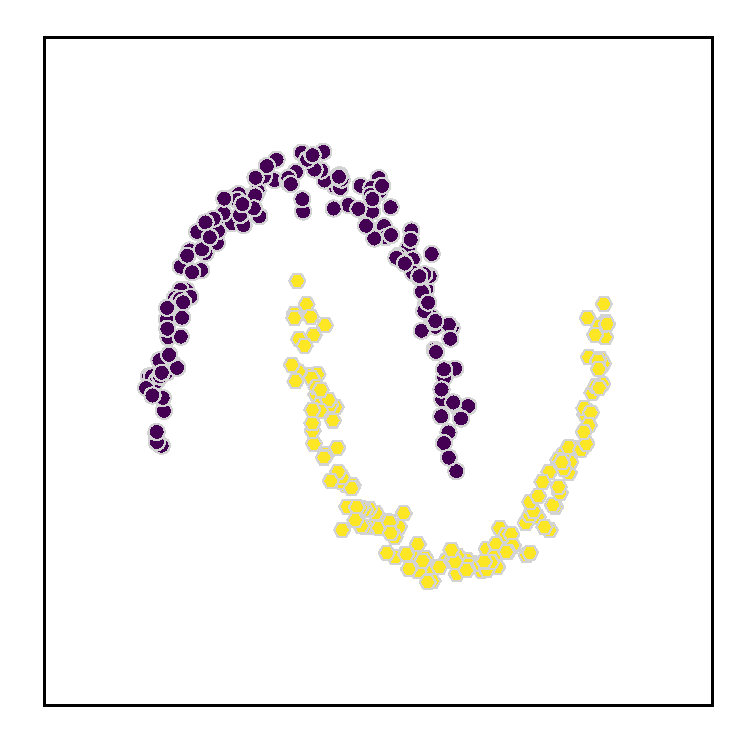
\includegraphics[width=\linewidth]{dbscan/moons}
        \caption{}\label{fig:dbscan_moons}
    \end{subfigure}%
    \hfill%
    \begin{subfigure}{.333\textwidth}
        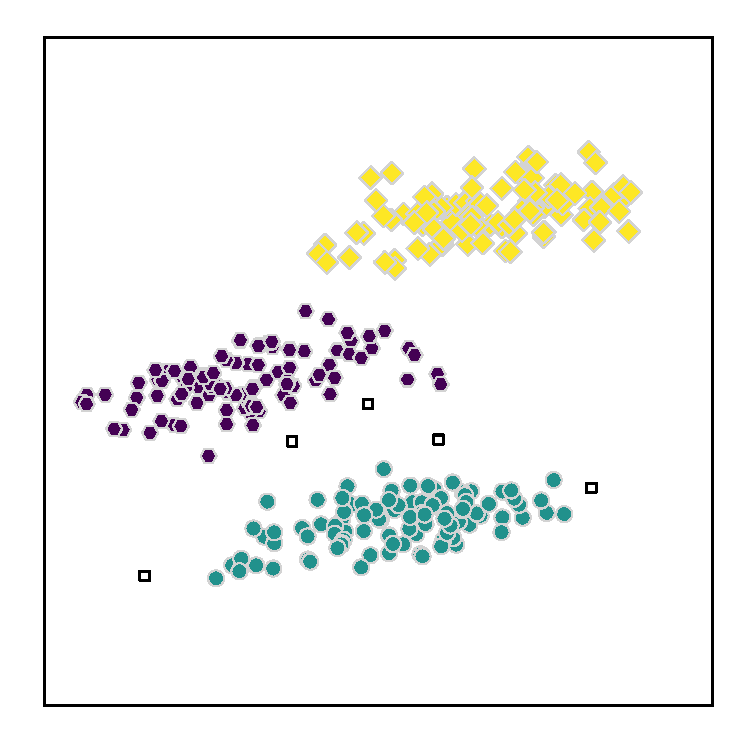
\includegraphics[width=\linewidth]{dbscan/ellipses}
        \caption{}\label{fig:dbscan_ellipses}
    \end{subfigure}%
    \hfill%
    \begin{subfigure}{.333\textwidth}
        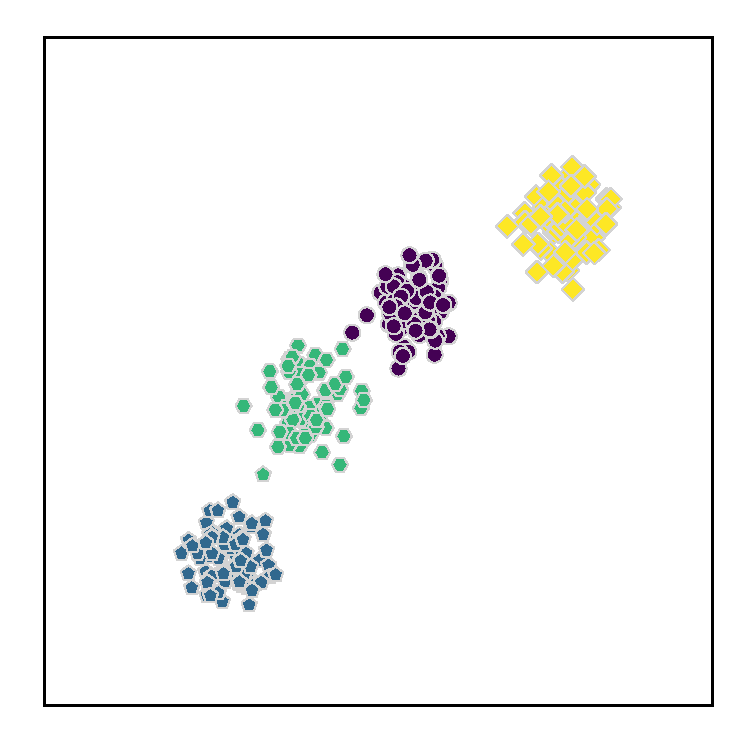
\includegraphics[width=\linewidth]{dbscan/spheres}
        \caption{}\label{fig:dbscan_spheres}
    \end{subfigure}
    \caption{%
        Clusters identified by DBSCAN on the (\subref{fig:dbscan_moons}) moons,
        (\subref{fig:dbscan_ellipses}) ellipses, and
        (\subref{fig:dbscan_spheres}) spheres datasets.%
    }\label{fig:dbscan_examples}
\end{figure}

Figure~\ref{fig:dbscan_examples} shows the equivalent plots to the other
paradigms discussed here, with the clustering being performed by the DBSCAN
algorithm. Unlike \(k\)-means or average-linkage, DBSCAN is able to identify the
crescent moon shapes in Figure~\ref{fig:dbscan_moons}. DBSCAN performs well at
clustering the globular datasets. However, Figure~\ref{fig:dbscan_ellipses}
exemplifies the sensitivity of DBSCAN and its parameters; a small number of
points have been deemed outliers with the particular value of \(\epsilon\) used
here. DBSCAN narrowly improves upon the hierarchical method for the spheres
dataset, but remains unable to correctly identify all of the data points.

\subsection{Healthcare modelling}\label{subsec:healthcare}

Healthcare modelling is a broad term that encompasses a plethora of techniques
from a number of disciplines such as financial modelling and forecasting, and
operational problems like vehicle routing or staff rostering. This review
focuses on these operational pursuits, and particularly those that are concerned
with patients directly. The decision to narrow the literature in this way is
both practical and conscientious, but an array of comprehensive reviews are
available, including~\cite{Brailsford2016,Galetsi2020,Kunc2018,Palmer2018}.
Practical by reducing the span of literature on `healthcare modelling' to
something less cumbersome, and conscientious as it allows this review to make a
small contribution to the research of the progressively more commonplace concept
of patient-centred care.

This form of healthcare, formally defined in~\cite{Robinson2008}, demands that
the perspective of a healthcare system should align itself with its patients'
needs and lived experiences. The alternative to patient-centred care would be a
system in which patients are treated in an exact but vague way, according to
only the needs of the system, say. Some form of patient-centred care has been
adopted in healthcare systems around the world including both state-funded and
private systems~\cite{DoH2010,Dewi2013,Luxford2011}. Unsurprisingly, its
application has been commended by patients, advocates and practitioners alike
for improving condition-specific
populations~\cite{Foster2019,Gambling2010,Gondek2016,Tsianakas2012} and more
broadly~\cite{IAPO2012,Richards2015,Santana2019}.

\subsubsection{Segmentation analysis}

Segmentation analysis allows for the targeted analysis of otherwise
heterogeneous datasets and encompasses several techniques from operational
research, statistics and machine learning. One of the most desirable qualities
of this kind of analysis is the ability to glean and communicate simplified
summaries of patient needs to stakeholders within a healthcare
system~\cite{Tomar2013,Vuik2016b,Yoon2020}. For instance, clinical profiling
often forms part of the broader analysis where each segment is summarised in a
phrase or infographic~\cite{Vuik2016a,Yan2019}.

The survey identified three commonplace groups of patient characteristics used
to segment a patient population: system utilisation metrics; clinical
attributes; and the pathway. The last is not used to segment the patients
directly, but instead groups patients' movements through a healthcare system;
this is typically done using a technique known as process mining. This technique
originates in business analytics, and has been used to study the efficiency of
hospital systems~\cite{Arnolds2018,Delias2015}. The remaining characteristics
can be segmented in a variety of ways, but recent works tend to favour
unsupervised methods --- typically latent class analysis (LCA) or
clustering~\cite{Yan2018}.

LCA is a statistical, model-based method used to identify groups (called latent
classes) in data by relating its observations to some unobserved (latent),
categorical attribute. This attribute has multiple possible categories, each
corresponding to a latent class. The discovered relations enable the
observations to be separated into latent classes according to their maximum
likelihood class membership~\cite{Hagenaars2002,Lazarsfeld1968}. This method has
proved useful in the study of comorbidity patterns (as
in~\cite{Kuwornu2014,Larsen2017}) where combinations of demographic and clinical
attributes are related to various subgroups of chronic diseases.

As demonstrated in Section~\ref{subsec:clustering}, clustering includes a wide
variety of methods where the common theme is to maximise homogeneity within, and
heterogeneity between, each cluster. Of those methods, \(k\)-means clustering
(or a variant thereof) is the most widely used in
healthcare~\cite{%
    Elbattah2017,Haraty2015,Ogbuabor2018,Santhi2010,Silitonga2018,Vuik2016a%
}; this is likely due to its simplicity and scalability. Hierarchical clustering
methods have also been applied to operational healthcare problems in recognising
patient utilisation patterns~\cite{Zayas2016}, profiling their healthcare
preferences~\cite{Liu2009}, and in mapping out effective healthcare leadership
models~\cite{Hargett2017}.

Furthermore, in \cite{Vuik2016a}, hierarchical clustering is utilised as a part
of the formative analysis, identifying a suitable number of clusters.  In
addition, supervised hierarchical segmentation methods such as classification
and regression trees (as in~\cite{Harper2006}) have been used where an existing,
well-defined label is of particular significance. An crucial and attractive
reason for using hierarchical methods in healthcare settings comes from the
dendogram visualisation. The use of effective visualisation tools encourages
(and allows, in some cases) involvement by key, expert stakeholders in the
simulation process. The same is true of \(k\)-means for its straightforward
construction. The authors of~\cite{Jahangirian2015} present a analysis of the
factors which result in a low level of engagement from stakeholders with
healthcare simulation work. The key findings indicate that complexity and
communication are the limiting factors for stakeholders, and so the onus resides
with researchers to make their models informative, effective and transferable.


\subsubsection{Queuing models}

Since the seminal works by Erlang~\cite{Erlang1917,Erlang1920} established the
core concepts of queuing theory, the application of queues and queuing networks
to real services has become abundant, including the healthcare service. By
applying these models to healthcare settings, many aspects of the underlying
system can be studied. A common area of study in healthcare settings is of
service capacity. The study~\cite{McClain1976} is an early example of such work
where acute bed capacity was determined using hospital occupancy data.
Meanwhile, more modern works consider more extensive sources of data to build
their queuing models~\cite{Palvannan2012,Pinto2014}. Moreover, the output of a
model is catered more towards being actionable --- as is the prerogative of
operational research. For instance, in~\cite{Pinto2014}, the authors devise new
categorisations for both hospital beds and arrivals that are informed by the
queuing model. A further example is~\cite{Komashie2015} where queuing models are
used to measure and understand satisfaction among patients and staff.

In addition to these theoretic models, healthcare queuing research has expanded
to include computer simulation models. The simulation of queues, or networks
thereof, have the benefit of adeptly capturing the stochastic nuances of
hospital systems over their theoretic counterparts. Example areas include the
construction and simulation of Markov processes via process
mining~\cite{Arnolds2018,Rebuge2012}, and patient flow~\cite{Bhattacharjee2014}.
Regardless of the advantages of simulation models, a prerequisite is reliable
software with which to construct those simulations. A common approach to
building simulation models of queues is to use a graphical user interface such
as Simul8. These tools are designed to be highly visual, making them attractive
to organisations looking to implement queuing models without necessary technical
expertise, including the NHS. The authors of~\cite{Brailsford2013} discuss the
issues around operational research and simulation being taken up in the NHS
despite the availability of intuitive software packages like Simul8.

However, they do not address a core principle of good simulation work:
reproducibility. The ability to reliably reproduce a set of results is of great
importance to scientific research but continues to be an issue in simulation
research generally~\cite{Fitzpatrick2019,Taylor2018}. When considering issues
with reproducibility in scientific computing (simulation included), the source
of any concerns is often with the software used~\cite{Ivie2018}. Using
well-developed, open-source software can alleviate issues around reproducibility
and reliability as how they are used involve less uncertainty and require more
rigour than `drag-and-drop' software. One example of such a piece of software is
Ciw~\cite{Palmer2019}. Ciw is a discrete event simulation library written in
Python that is fully documented and tested.

% TODO discussion of multiclass queuing models and lack of integration with
% clustering

\subsection{Evaluating a model}

In~\cite{Caswell1976}, the author presents a seminal work discussing the proper
evaluation of scientific models, drawing attention to a component of modelling
that (even now) is often skimmed over. The author establishes a need for a clear
distinction between \emph{validation} and \emph{corroboration} when evaluating a
model; given that a model characterises a part of a wider reality through some
parameterisation, no model can be `valid', i.e. true. Instead, a model can be
\emph{confirmed} and support some hypothesis about the reality which it models.
This sentiment is echoed by the adage, `all models are wrong, but some are
useful'~\cite{Box1979}, in that good models can and should illuminate a
particular research problem. Works of this era raise important points,
cautioning researchers about relying too heavily on their models, but the
question still stands: how can (and should) a model be evaluated?

With the large-scale use of electronic data and the advent of computer
simulation models, the importance of this question grows. The authors
of~\cite{Oreskes1994} presented a landmark work that reiterates the concerns of
earlier works, framing the question of model evaluation more squarely for
computer simulation models. Again, one focus of~\cite{Oreskes1994} is on the use
of particular language when discussing the quality of a model, i.e. no model can
be validated, but rather a model can be confirmed when its output aligns with
some observed data. The authors go a step further in stating that any
corroborative support offered by model confirmation is `inherently partial'
given the assumptions made to construct a model. However, this confirmation
process has become the standard response for evaluating computer simulation
models --- choose a metric and dataset (or sets thereof) use these to quantify
the quality of the model either alone or against some competitor(s).

These works indicate that the evaluation of a model should not be purely
mathematical or practical, and as such, it invokes a need for some philosophical
thinking. In~\cite{Parker2010}, the author consolidates the concerns of
practitioners and philosophers regarding model evaluation, defining scientific
models as representational tools constructed to achieve a particular purpose or
goal; earlier and more contemporary works concur with this
definition~\cite{Baumberger2017,Caswell1976,Currie2017}. The author suggests
that model evaluation should be considered as the process of determining whether
a model is \emph{adequate} for a purpose, i.e. whether a model is highly likely
to achieve a goal. The author distinguishes this concept of adequacy and from
individual success where a model achieves a purpose in a particular instance.

Later, in~\cite{Parker2020}, the same author elaborates on this
adequacy-for-purpose view of model evaluation, highlighting the contrasts
between determining adequacy of a model and measuring the accuracy of its
representation against some target. In particular, the author emphasises the
real-world dangers of overconfidence in a model's performance against any
confirmation process. By defining models as tools constructed from parameters
and simplifications, they are not generally boolean. Therefore, in general, they
cannot be the subject of true confirmation. However, in practice, if a model is
accredited through some confirmation process, the general merit and confidence
in that model increases, potentially leading to the collective idea that the
model has been `confirmed' and may be `better' than some other(s) without regard
for its assumptions or limitations.

The author offers four practical methods for assessing adequacy-for-purpose that
address evaluation at the point of model construction, and as a part of post hoc
analysis. However, they conclude by recommending that any sufficient assessment
suite should include a synthesis of the presented strategies, leaving open
questions regarding the criteria of how each assessment should be aggregated to
form a single conclusion. The author presents several examples and addresses
potential concerns, demonstrating that the rigorous evaluation of any model
requires careful, measured processes.

One quick alternative to this due diligence is to rephrase a purpose in terms of
a reasonable limit on some criterion. For instance, rather than asking whether a
method is adequate for predicting some quantity, the purpose could be rephrased
as `predicting some quantity with an accuracy of \(x\)\%'. In these terms, the
power of the statement is diminished, but practically, this question becomes
much more straightforward to answer. In addition, rephrasing the purpose in this
way results in a conclusion which is broadly equivalent to a confirmation
process, indicating little about the true quality or robustness of the method.

So, while these works are highly valuable in expanding the discussion of model
evaluation, without concrete and readily applied methods with which to quantify
their approaches, they are unlikely to be adopted widely. This unlikelihood is
not necessarily the fault of the methods, but rather that (in some respects)
convenience and velocity have surpassed merit in the evaluation of models. In an
increasingly competitive environment where becoming the new `state-of-the-art'
has become the norm, regard for robust, thoroughly evaluated models has
declined. The remainder of this section summarises the established evaluation
processes for clustering algorithms and healthcare models, highlighting their
limitations and potential improvements to the current regime.

\begin{itemize}
    \item Objectivity vs. fairness
    \item Human intervention
    \item Unconscious bias
\end{itemize}

\subsubsection{Clustering}

Algorithms for clustering, like many machine learning tasks, fall into the
category of models that are primarily evaluated using confirmation processes. To
reiterate, a confirmation process provides support for a model based on its
alignment with a set of observed data according to some metric. Often lumped in
with the task of classification, clustering is distinct in that it reveals the
underlying structure of a dataset with knowledge that is fixed from the outset
exclusively. However, the metrics used to evaluate clustering algorithms are
often concerned with the retrieval of information such as accuracy, precision,
and recall~\cite{Manning2008}. Examples of this method of evaluation are
abundant, including many of the cited works from Section~\ref{subsec:clustering}
such as~\cite{Agrawal1998,Aljarah2019,Bakr2015,Cao2009,Huang1998}.

Information retrieval metrics can be considered \emph{external criteria} in that
they measure an aspect of a model's clustering according to a external labelling
of the dataset~\cite{Mitchell1997}. By evaluating a clustering algorithm based
on a ground truth, the algorithm is effectively being evaluated as a classifier
--- a method which is trained using that ground truth. Hence, the quality of any
clustering is predicated on the data generation process, and if a clustering
algorithm cannot replicate the external labelling, it will not be deemed fit
using external, label-dependent criteria. When discussing the demonstrative
figures in Section~\ref{subsec:clustering}, an informal form of this evaluation
was made when referring to a `mislabelling' of points. In reality, the data
synthesis produced a structure within the data that is not necessarily congruent
with the generative process. Therefore, the clustering algorithms (which
identify unknown structures) should not be penalised for not recognising these
anomalies.

Without the use of an external truth, \emph{internal criteria} exist to evaluate
clustering algorithms. A criterion is considered internal if its sole source of
information is the clustering produced by the algorithm. For centroid-based and
divisive clustering algorithms, a common internal measure is the inertia of a
clustering, i.e. some loss function regarding the cluster
centres~\cite{Everitt2011}. Using inertia as a quality measure is convenient
given that practical implementations of centroid-based methods use inertia as
their objective function, meaning it is readily available. However, interpreting
inertia values can be difficult as it is scale-variant. As such, the inertia can
be presented as a normalised measure using the all-cluster loss (i.e. the
inertia when all points are contained in a single cluster), for instance.

Another popular internal quality measure is the silhouette
coefficient~\cite{Rousseeuw1987} which presents a ratio between the tightness
and separation of a set of clusters. This measure has the benefit of taking
values in a finite range (from \(-1\) to \(1\)), making it interpretable across
several methods. Furthermore, it does not rely on cluster centres, and so can be
applied to other clustering
paradigms~\cite{Garcia2011,Guan2019,Starczewski2015}. However, the primary
drawback of the silhouette coefficient (as with inertia) is that it strongly
favours linearly separable, spherical clusters. The authors
of~\cite{Frederix2004} present two cluster-quality measures that avoid this
bias, but rely on knowing the `true' clusters of a dataset.

Further to particular metrics --- objective or otherwise --- clustering
evaluation has been generalised to study more intrinsic properties of clustering
instances such as clusterability~\cite{Ackerman2009,Ostrovsky2006,Zhang2001}.
These works often rely on an axiomatic description of clustering (examples of
which include~\cite{Bezdek1978,Jardine1971,Kleinberg2002}).
In~\cite{Kleinberg2002}, the author presents a theorem stating that no
clustering function (i.e. a function that partitions a set of points according
to a distance measure) exists which satisfies all three of the following
axiomatic properties: 

\begin{itemize}
    \item Scale-invariance: the function is insensitive to changes in the unit
        distance
    \item Richness: all partitions of the dataset are possible outputs of the
        function (by use of an alternative distance function)
    \item Consistency: the outputted clustering is unchanged when within-cluster
        distances are decreased and between-cluster distances are increased
\end{itemize}

However, small changes to these properties accommodate various well-known
clustering algorithms, including single-linkage and \(k\)-means (discussed in
Section~\ref{subsec:clustering}). The authors of~\cite{BenDavid2008} expand on
these axioms to derive necessary and desirable properties of cluster-quality
measures that are entirely agnostic to the clustering function at hand. The
closing sections of that work offer a number of exemplar cluster-quality
measures based on loss, cluster centres and linkage, including measures that
correspond to the all-cluster normalised mean-squared error, and a
within-versus-between variability measure. The latter can be considered as a
generalisation of the silhouette coefficient that is invariant to its loss
function or distance measure.

\begin{itemize}
    \item fair clustering methods
    \item benchmark datasets (often classification datasets)
    \item synthetic datasets (benchmarks(?), how are they made?)
\end{itemize}

\subsubsection{Healthcare settings}

\begin{itemize}
    \item often dependent on model
    \item incorporating staff and patient feedback
    \item where is model accountability?
\end{itemize}
